\documentclass[11pt,onecolumn]{article}
\setlength{\columnsep}{0.5cm}

\usepackage[utf8]{inputenc}
\usepackage[T1]{fontenc}
\usepackage[spanish]{babel}
\usepackage{hyperref}
\usepackage{graphicx}
\usepackage{natbib}
\usepackage{rotating}

\title{\vspace{-15mm}%
	\fontsize{24pt}{10pt}\selectfont
	\textbf{Estado del arte de la investigación sobre wikis}
	}	
\author{%
	\large
	\textsc{Emilio J. Rodríguez-Posada} \\
	\normalsize	Universidad de Cádiz \\
	\normalsize	\href{mailto:emiliojose.rodriguez@uca.es}{emiliojose.rodriguez@uca.es}
	\vspace{-5mm}
	}
\date{}


\begin{document}

\maketitle

\begin{abstract}

\end{abstract}

\section{Introducción}

En principio lo que voy a hacer es analizar el estado del arte de la investigación de wikis, contar WikiPapers, y un poco de mi trayectoria en estos temas, cuestiones abiertas, conclusiones y trabajo futuro.

Quizás para que fuera abordable el estado del arte, podría limitarme a clasificar los papers del último o dos últimos WikiSym. Y al último PAN/CLEF, WikiAI, MathWikis, Wikimania, WikiViz, etc. Comentar la existencia de todos estos eventos.

Reutilizar cosas que haya escrito ya en mis papers.

La intro la puedo adaptar del SLR que estoy haciendo de WikiPapers

\section{Motivación}

\section{Objetivos}

Hacer un estado del arte


\section{Definiciones, acrónimos y abreviaturas}

Mirar las que definí en mi PFC y meter otras más nuevas

\textbf{Administrador}:

\textbf{Anónimo}:


\textbf{API}:

\textbf{Artículo}:

\textbf{Blanqueo}:

\textbf{Bloqueo}:

\textbf{Bot}:

\textbf{Cambios recientes}:

\textbf{Cultura libre}:


\textbf{Dataset}:

\textbf{Diff}:


\textbf{Discusión}:

\textbf{Edición}:

\textbf{Espacio de nombres}:

\textbf{Etiqueta}:

\textbf{Expresión regular}:

\textbf{Fork}:


\textbf{GLAM}:

\textbf{Historial}:

\textbf{Interwiki}:

\textbf{Los cinco pilares}:


\textbf{Motor wiki}:

\textbf{Namespace}: véase \textbf{Espacio de nombres}.

\textbf{NPOV}: véase \textbf{Punto de vista neutral}.

\textbf{Política}:

\textbf{Preservación}:

\textbf{Proyectos hermanos}:

\textbf{Punto de vista neutral}:

\textbf{Regexp}: véase \textbf{Expresión regular}.

\textbf{Resumen de edición}:


\textbf{Reversión}:

\textbf{Robot}:


\textbf{Semántica}:

\textbf{Spam}:


\textbf{Usabilidad}:

\textbf{Vandalismo}:

\textbf{Web 2.0}:

\textbf{Wiki}:

\textbf{Wikifarm}:


\section{Estado del arte}

Áreas de investigación \href{http://wikipapers.referata.com/wiki/List_of_research_areas}{http://wikipapers.referata.com/wiki/List\_of\_research\_areas}

~\citep{okoli2009}
~\citep{martin2011}
~\citep{voss2005}
~\citep{okoli2009b}
~\citep{ayers2006}
~\citep{okoli2012}
~\citep{jullien2012}
~\citep{nielsen2011}


\subsection{Autoría y calidad}

WikiTrust, comparación Nature


\subsection{Cobertura y sesgos}


\subsection{Comunidad}


\subsection{Educación}


Wikis como herramientas educativas

Experiencias docentes

\subsection{Datasets}

\href{http://wikipapers.referata.com/wiki/List_of_datasets}{http://wikipapers.referata.com/wiki/List\_of\_datasets}

\begin{sidewaystable}[h]
\centering
\begin{tabular}{| c | c | c | c |}
\hline
\textbf{Dataset} & \textbf{Tamaño} & \textbf{Idioma} & \textbf{Descripción} \\
\hline
CoCoBi & · & Alemán & · \\ \hline 
Coordinates in Wikipedia articles & · & Multilingüe & · \\ \hline 
DBpedia & · & Multilingüe & · \\ \hline 
DeletionPedia & · & Inglés & · \\ \hline 
Domas visits logs & · & Multilingüe & · \\ \hline 
Google dataset linking strings and concepts & · & Multilingüe & · \\ \hline 
PAN Wikipedia vandalism corpus 2010 & · & Inglés & · \\ \hline 
PAN Wikipedia vandalism corpus 2011 & · & Multilingüe & · \\ \hline 
PlusPedia & · & Alemán & · \\ \hline 
Repos-2012-dataset & · & Multilingüe & · \\ \hline 
Social networks of Wikipedia dataset & · & · & · \\ \hline 
WikiBiography & · & · & · \\ \hline 
WikiCorpus & · & Multilingüe & · \\ \hline 
WikiIndex & · & Inglés & · \\ \hline 
WikiNet & · & Multilingüe & · \\ \hline 
WikiPapers & · & Inglés & · \\ \hline 
WikiRelations & · & Inglés & · \\ \hline 
WikiTaxonomy & · & · & · \\ \hline 
WikiTeam dumps & · & Multilingüe & · \\ \hline 
Wikia dumps & · & Multilingüe & · \\ \hline 
Wikimedia dumps & · & Multilingüe & · \\ \hline 
Wikipedia Historical Attributes Data & · & Inglés & · \\ \hline 
Wikipedia Vandalism Corpus (West) & · & Inglés & · \\ \hline 
Wikipedia page-to-page link database & · & Inglés & · \\ \hline 
WikipediaXML & · & Multilingüe & · \\ \hline 
Wlm-2011-dataset & · & Multilingüe & · \\ \hline
\end{tabular}
\caption{Datasets relacionados con wikis.}
\label{tab:datasetstable}
\end{sidewaystable}

\subsection{GLAM}


\subsection{Herramientas}

\href{http://wikipapers.referata.com/wiki/List_of_tools}{http://wikipapers.referata.com/wiki/List\_of\_tools}

\begin{sidewaystable}[h]
\centering
\begin{tabular}{| c | c | c | c | c |}
\hline
\textbf{Herramienta} & \textbf{S.O.} & \textbf{Idioma} & \textbf{Licencia} & \textbf{Descripción} \\
\hline
AVBOT & Multiplataforma & Español & GPL & Bot anti-vandalismo para Wikipedia en español. \\ \hline
ClueBot & GNU/Linux & · & · & · \\ \hline
CryptoDerk's Vandal Fighter & Multiplataforma & Inglés & · & · \\ \hline
Huggle & Windows & · & GPL & · \\ \hline
Igloo & · & · & · & · \\ \hline
STiki & Multiplataforma & Inglés & GPL & · \\ \hline
Salebot & · & · & · & · \\ \hline
Twinkle & · & · & · & · \\ \hline
Vandal Fighter & Multiplataforma & Inglés & · & · \\ \hline
VandalProof & Windows & Inglés & · & · \\ \hline
VandalSniper & Multiplataforma & Inglés & · & · \\ \hline
\end{tabular}
\caption{Herramientas anti-vandalismo y anti-spam.}
\label{tab:vandaltoolstable}
\end{sidewaystable}


\begin{sidewaystable}[h]
\centering
\begin{tabular}{| c | c | c | c | c |}
\hline
\textbf{Herramienta} & \textbf{S.O.} & \textbf{Idioma} & \textbf{Licencia} & \textbf{Descripción} \\
\hline
Java Wikipedia Library & Multiplataforma & Inglés & LGPL & Framework en Java. \\ \hline
Perlwikipedia & Multiplataforma & Inglés & GPL & Framework en Perl. \\ \hline
Python-wikitools & Multiplataforma & Inglés & GPL & Framework en Python. \\ \hline
Pywikipediabot & Multiplataforma & Inglés & MIT license & Frame work en Python. El más usado. \\ \hline
\end{tabular}
\caption{Frameworks.}
\label{tab:frameworkstable}
\end{sidewaystable}


\begin{sidewaystable}[h]
\centering
\begin{tabular}{| c | c | c | c | c |}
\hline
\textbf{Herramienta} & \textbf{S.O.} & \textbf{Idioma} & \textbf{Licencia} & \textbf{Descripción} \\
\hline
JWordNet-Similarity & Multiplataforma & Inglés & · & · \\ \hline 
Manypedia.com & Multiplataforma & Inglés & Affero GPL & · \\ \hline 
Wikokit & Multiplataforma & Inglés & Varias & · \\ \hline 
Zawilinski & Multiplataforma & · & · & · \\ \hline 
\end{tabular}
\caption{Herramientas sobre el lenguaje.}
\label{tab:languagetoolstable}
\end{sidewaystable}


\begin{sidewaystable}[h]
\centering
\begin{tabular}{| c | c | c | c | c |}
\hline
\textbf{Herramienta} & \textbf{S.O.} & \textbf{Idioma} & \textbf{Licencia} & \textbf{Descripción} \\
\hline
DiffDB & · & · & · & · \\ \hline 
Ikiwiki & · & · & · & · \\ \hline 
Infobox2rdf & · & · & · & · \\ \hline 
MediaWiki API & · & · & · & · \\ \hline 
Sioc MediaWiki & · & · & · & · \\ \hline 
Wiki Edit History Analyzer & · & · & · & · \\ \hline 
Wiki2XML parser & · & · & · & · \\ \hline 
WikiPrep & · & · & · & · \\ \hline 
Wikihadoop & · & · & · & · \\ \hline 
Wikimedia Utilities & · & · & · & · \\ \hline 
Wikipedia Extractor & · & · & · & · \\ \hline 
Wikipedia Miner & · & · & · & · \\ \hline 
Wikipedia-map-reduce & · & · & · & · \\ \hline 
\end{tabular}
\caption{Herramientas de procesamiento de datos.}
\label{tab:dataprocessingtoolstable}
\end{sidewaystable}


\begin{sidewaystable}[h]
\centering
\begin{tabular}{| c | c | c | c | c |}
\hline
\textbf{Herramienta} & \textbf{S.O.} & \textbf{Idioma} & \textbf{Licencia} & \textbf{Descripción} \\
\hline
HistoryFlow & · & · & · & · \\ \hline 
StatMediaWiki & · & · & · & · \\ \hline 
Wiki Explorator & · & · & · & · \\ \hline 
Wiki Trip & · & · & · & · \\ \hline 
WikiBlame & · & · & · & · \\ \hline 
WikiChanges & · & · & · & · \\ \hline 
WikiEvidens & · & · & · & · \\ \hline 
WikiPride & · & · & · & · \\ \hline 
WikiScanner & · & · & · & · \\ \hline 
WikiTracer & · & · & · & · \\ \hline 
WikiTrust & · & · & · & · \\ \hline 
WikiVis (FH-KL) & · & · & · & · \\ \hline 
WikiVis (UM) & · & · & · & · \\ \hline 
WikiWarMonitor & · & · & · & · \\ \hline 
WikiXRay & · & · & · & · \\ \hline 
Wikistream & · & · & · & · \\ \hline 
Wmcharts & · & · & · & · \\ \hline 
\end{tabular}
\caption{Herramientas de visualización.}
\label{tab:visualizationtoolstable}
\end{sidewaystable}


\begin{sidewaystable}[h]
\centering
\begin{tabular}{| c | c | c | c | c |}
\hline
\textbf{Herramienta} & \textbf{S.O.} & \textbf{Idioma} & \textbf{Licencia} & \textbf{Descripción} \\
\hline
WikiSim & · & · & · & · \\ \hline 
WikiTeam tools & · & · & · & · \\ \hline 
· & · & · & · & · \\ \hline 
\end{tabular}
\caption{Otras herramientas.}
\label{tab:othertoolstable}
\end{sidewaystable}



\subsection{Historiales}


\subsection{Infraestructura}

por ejemplo los wikis al estilo p2p para repartir la carga... había una tesis sobre eso en danés?


\subsection{Motivaciones e incentivos}


Encuestas...

\subsection{Motores wiki}


\subsection{Preservación}

urobe, revisar el paper de wikiteam

\subsection{Procesamiento de imágenes}

Poquísimo hay hecho me parece a mí...

\subsection{Procesamiento del Lenguaje Natural}


\subsection{Recomendación de tareas}

Images for bio

\subsection{Semántica}

SWEETpedia

\subsection{Usabilidad}


\subsection{Vandalismo y spam}

Bots y algoritmos, flaggedrevs, abusefilter, extensiones anti-spam

~\citep{avbot2011}
~\citep{avbot2010}
~\citep{avbot2009}

\subsection{Visualización}

WikiViz y todas las herramientas de visualización...


\subsection{Wikifarms}

~\citep{kittur2010}

\subsection{Wikis como redes sociales}


\section{Cuestiones abiertas}


\begin{figure}[htb]
\centering
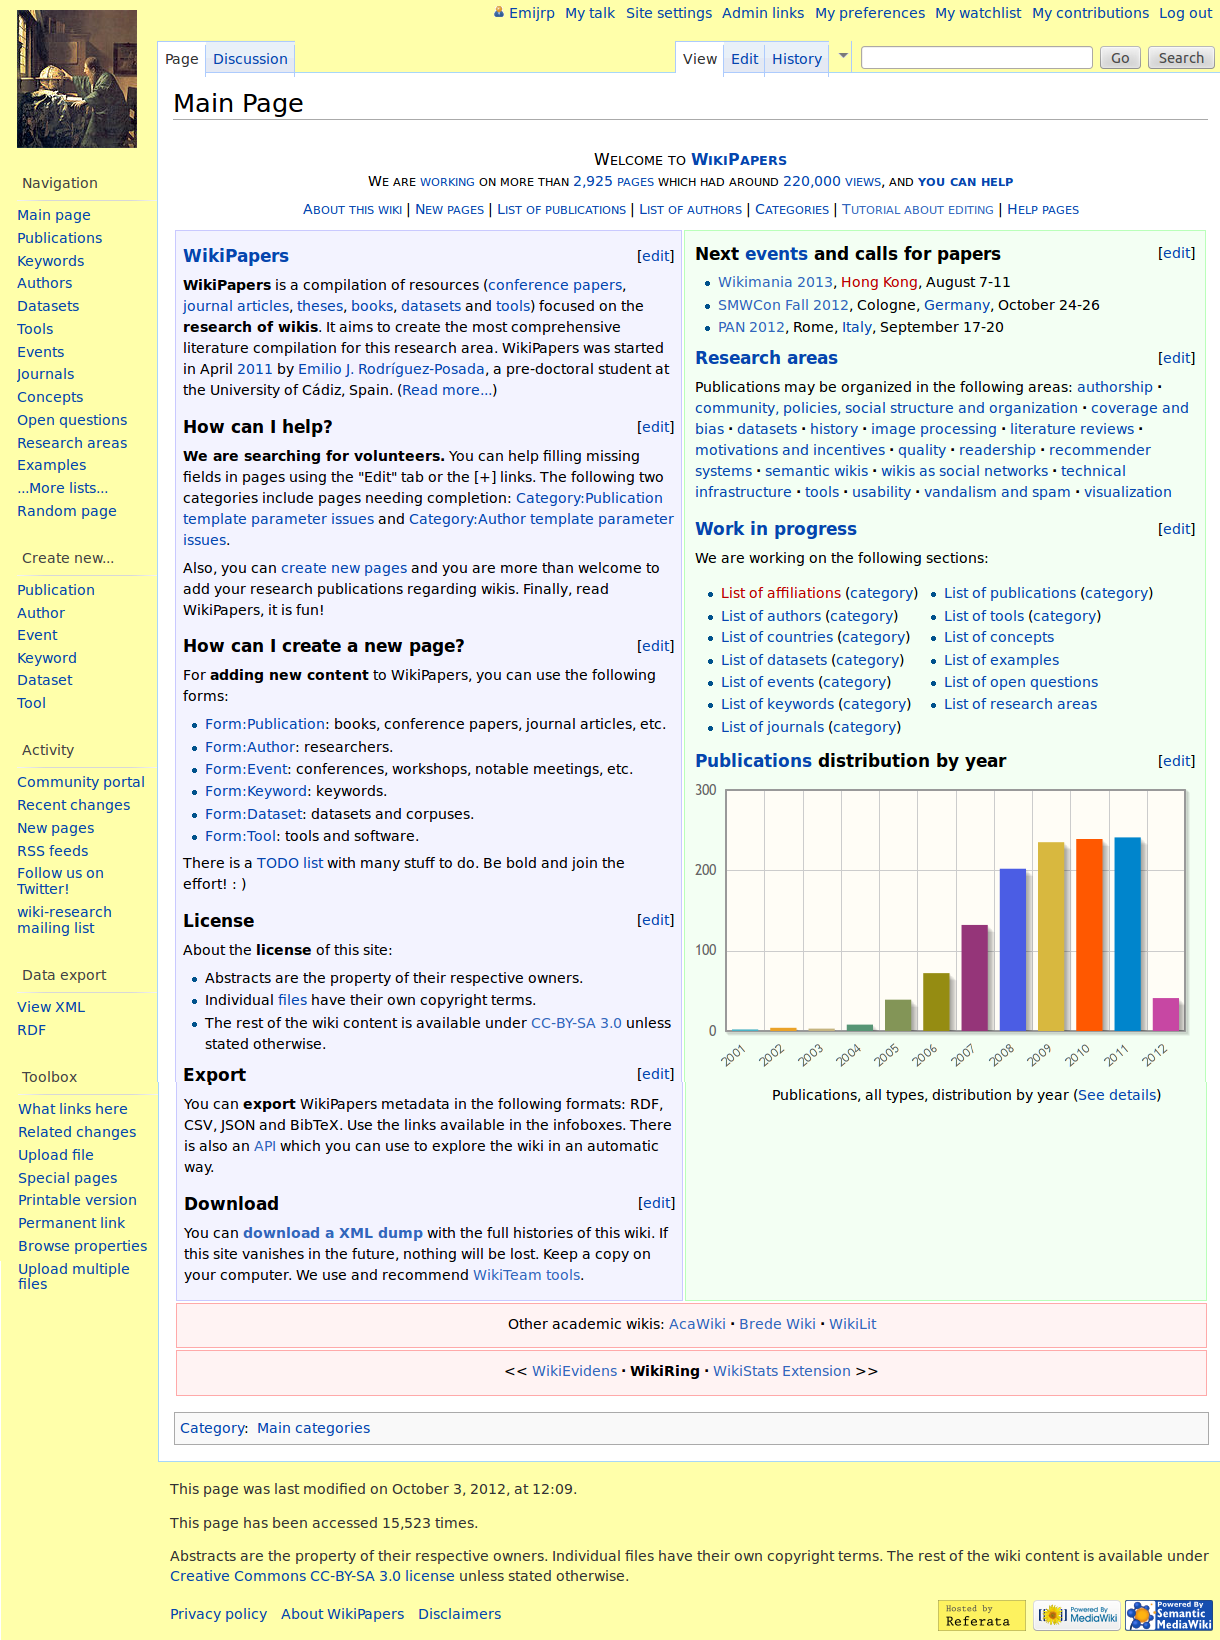
\includegraphics[width=0.8\textwidth]{wpfull.png}
\caption{Portada de WikiPapers}
\label{fig:wpfull}
\end{figure}


\section{Conclusiones y trabajo futuro}
porqué hacía falta WikiPapers
aglutina todas las ventajas de los anteriores sistemas
lo que se ha hecho, cifras,
lo que queda por hacer y como ayudar
el futuro y más allá...



\bibliographystyle{wink}        
\bibliography{proyecto-investigacion-2012}

\section*{Licencia}
Esta obra está bajo licencia \href{http://creativecommons.org/licenses/by-sa/3.0/}{Creative Commons Reconocimiento-CompartirIgual 3.0 Unported}.

\end{document}
